% Original mechanism workshop; qualitative energy sketches are not measured energy data.
\documentclass[11pt,aspectratio=169]{beamer}
\usetheme{Darmstadt}
\usecolortheme{rose}
\usepackage[version=4]{mhchem}
\usepackage{chemfig,tikz,booktabs}
\usetikzlibrary{arrows.meta}
\setbeamercolor{structure}{fg=red!65!black}
\setbeamertemplate{navigation symbols}{}
\title{Follow the electrons}
\subtitle{Choosing between a concerted substitution and an ionization pathway}
\author{Organic chemistry workshop}
\date{Mechanism clinic 09}
\begin{document}
\begin{frame}[plain]\titlepage\end{frame}
\section{Notice}
\begin{frame}{Inspect the reacting centre before naming a mechanism}
\begin{columns}[c]
\begin{column}{.45\textwidth}\centering
\chemfig{CH_3-CH_2-Br}
\bigskip\par
{\footnotesize\ce{HO^- + CH3CH2Br -> CH3CH2OH + Br^-}}
\end{column}
\begin{column}{.5\textwidth}
\begin{enumerate}[<+->]
\item Locate the carbon attached to the leaving group.
\item Identify the electron-pair donor.
\item Ask what other pathways the conditions permit.
\end{enumerate}
\end{column}
\end{columns}
\end{frame}
\section{Draw}
\begin{frame}{An electron arrow starts at electrons}
\framesubtitle{A schematic for bond making and bond breaking in one step}
\centering
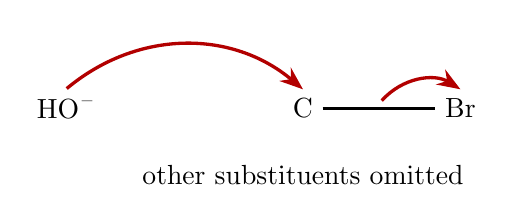
\begin{tikzpicture}[>=Stealth]
\node (nu) at (0,0) {\ce{HO^-}};
\node (c) at (3,0) {$\mathrm{C}$};
\node (br) at (5,0) {$\mathrm{Br}$};
\draw[thick] (c)--(br);
\draw[->,very thick,red!70!black] (nu.north) to[bend left=40] (c.north);
\draw[->,very thick,red!70!black] (4,.1) to[bend left=40] (br.north);
\node[below] at (3,-.6) {other substituents omitted};
\end{tikzpicture}
\begin{block}{Bookkeeping}
One pair forms the new bond; the old carbon--bromine bond pair goes to bromine. Check charge and valence on both sides.
\end{block}
\end{frame}
\begin{frame}{A rate law can distinguish proposed elementary pictures}
\begin{table}\centering
\begin{tabular}{lll}\toprule
Model & Rate expression & Elementary picture\\\midrule
$\mathrm{S_N2}$ & $k[\mathrm{RX}][\mathrm{Nu}]$ & concerted displacement\\
$\mathrm{S_N1}$ & $k[\mathrm{RX}]$ & rate-limiting ionization\\\bottomrule
\end{tabular}
\caption{Idealized kinetic descriptions; observed chemistry may include competing pathways.}
\end{table}
\pause
\alert{Prompt:} at fixed substrate concentration, what would doubling the nucleophile concentration test?
\end{frame}
\section{Compare}
\begin{frame}{A qualitative energy landscape is a mechanism proposal}
\begin{columns}[T]
\begin{column}{.48\textwidth}
\centering\textbf{One transition state}
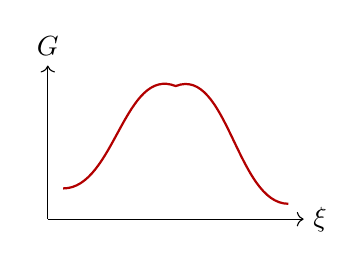
\begin{tikzpicture}[scale=.65]
\draw[->] (0,0)--(5,0) node[right]{$\xi$};\draw[->] (0,0)--(0,3) node[above]{$G$};
\draw[thick,red!70!black] (.3,.6)..controls(1.3,.6)and(1.5,3)..(2.5,2.6)..controls(3.5,3)and(3.7,.3)..(4.7,.3);
\end{tikzpicture}
\end{column}
\begin{column}{.48\textwidth}
\centering\textbf{An intermediate}
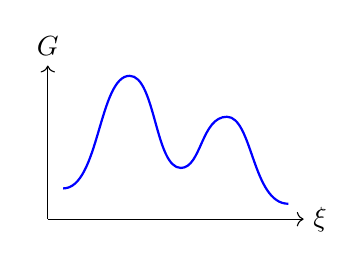
\begin{tikzpicture}[scale=.65]
\draw[->] (0,0)--(5,0) node[right]{$\xi$};\draw[->] (0,0)--(0,3) node[above]{$G$};
\draw[thick,blue] (.3,.6)..controls(1,.6)and(1,2.8)..(1.6,2.8)..controls(2.1,2.8)and(2.1,1)..(2.6,1)..controls(3,1)and(3,2)..(3.5,2)..controls(4,2)and(4,.3)..(4.7,.3);
\end{tikzpicture}
\end{column}
\end{columns}
\small Curves are qualitative teaching sketches. Reaction coordinate $\xi$ is not elapsed time; barrier heights are not to scale.
\end{frame}
\begin{frame}{Build a conditional decision table}
\begin{description}
\item[Substrate] Steric accessibility matters for backside attack.
\item[Solvent] Stabilization of ions and of the nucleophile can change pathway competition.
\item[Reagent] Basicity and nucleophilicity are related but distinct questions.
\item[Temperature] Evaluate elimination alongside substitution.
\end{description}
No single row replaces a complete analysis of substrate and conditions.
\end{frame}
\section{Explain}
\begin{frame}{Stereochemistry is a test of the proposed path}
\begin{block}{Concerted backside displacement}
At a stereogenic reacting centre, the $\mathrm{S_N2}$ geometry gives inversion of configuration.
\end{block}
\begin{alertblock}{A careless shortcut}
Do not turn ``a planar carbocation permits attack from either face'' into a universal prediction of an exactly racemic measured product. Ion pairing and the surrounding environment can matter.
\end{alertblock}
\end{frame}
\begin{frame}{Workshop task: defend the arrows, not the label}
\begin{enumerate}
\item Draw the proposed elementary steps and every formal charge.
\item Predict one kinetic observation.
\item Predict one stereochemical observation when applicable.
\item Name a competing pathway and an observation that would favour it.
\end{enumerate}
\bigskip
A useful mechanism makes a checkable prediction.
\end{frame}
\begin{frame}{Reading and representation}
\small
Background: MIT OpenCourseWare, \href{https://ocw.mit.edu/courses/5-12-organic-chemistry-i-spring-2003/pages/calendar/}{\emph{Organic Chemistry I}, lectures 13--15 on substitution}.
\medskip
The substrates, prompts, arrow schematic and qualitative energy drawings in this deck are original. The schematic omits substituents intentionally; it is not a complete stereochemical drawing. Reaction equations use \texttt{mhchem}; structural formulae use \texttt{chemfig}.
\end{frame}
\end{document}
